\section{결과와 분석}\label{sec:results}
\subsection{여러 기반 추정기에서의 보정 효과}
표~\ref{tab:backbones}는 같은 319장에 대한 각 기반의 Base와 N3를 비교한다. 코너 오차 중앙값은 YOLO에서 6.721에서 5.778픽셀, DOPE에서 12.570에서 7.469픽셀, ResNet에서 8.223에서 7.085픽셀로 감소하였다. \pckten 도 각각 63.425\%에서 68.587\%, 24.170\%에서 44.338\%, 52.261\%에서 57.223\%로 증가하였다. 동일 보정 절차를 기반별로 학습했을 때 초기 코너의 중심부 정확도와 전체 주석 기준 성공 코너 비율이 개선되었다.

위치·회전 중앙값의 점추정도 세 기반에서 감소하였다. 표~\ref{tab:pose_uncertainty_main}에서 YOLO와 DOPE의 두 중앙값 변화는 사후 세션 구간에서도 음수였다. 반면 ResNet의 위치 중앙값 차이 구간은 $[-2.077,0.202]$cm로 0을 포함한다. 세 기반의 점추정 감소를 모든 자세량의 확증적 개선으로 해석하지 않는다. 전체 P90·방향각 구간과 seed별 편차는 보충자료에 제시한다.
\begin{table*}[t]
\centering\footnotesize
\setlength{\tabcolsep}{4pt}
\caption{세 기반 추정기의 보정 전후. 같은 기반 안의 동일 초기 출력에 N3를 적용한다. 조건부 자세 통계의 분모가 기반별로 달라 기반 간 순위표가 아니다.}\label{tab:backbones}
\begin{tabularx}{\textwidth}{Ylrrrrrrrr}
\toprule
기반 & 경로 & \shortstack{코너 중앙값\\(px)} & \shortstack{코너 P90\\(px)} & \shortstack{\pckten\\(\%)} & \shortstack{위치 중앙값\\(cm)} & \shortstack{회전 중앙값\\(도)} & \shortstack{2D 매칭\\영상} & \shortstack{유효 예측\\코너} & \shortstack{자세 산출\\(\%)} \\
\midrule
YOLO & Base & 6.721 & 43.890 & 63.425 & 7.897 & 2.539 & 311/319 & 2,445 & 100.00 \\
YOLO & N3 & 5.778 & 42.134 & 68.587 & 7.068 & 2.070 & 311/319 & 2,445 & 100.00 \\
DOPE & Base & 12.570 & 51.282 & 24.170 & 10.046 & 3.530 & 233/319 & 1,797 & 65.83 \\
DOPE & N3 & 7.469 & 53.570 & 44.338 & 8.356 & 3.051 & 233/319 & 1,797 & 65.83 \\
ResNet-18$^\dagger$ & Base & 8.223 & 62.638 & 52.261 & 9.739 & 4.342 & 292/319 & 2,291 & 100.00 \\
ResNet-18$^\dagger$ & N3 & 7.085 & 62.371 & 57.223 & 9.134 & 3.832 & 292/319 & 2,291 & 100.00 \\
\bottomrule
\end{tabularx}
\tabnote{전체 319장·참조 2,499코너. 코너 중앙값·P90은 유효 매칭 코너에, 위치·회전은 산출된 자세에 조건부이다. YOLO Base/N3 자세는 전체 319/319장이며 2D 매칭 311/319장과 구분한다. N3는 세 seed의 통계 평균이며 앙상블이 아니다. $^\dagger$10-epoch CONSTANT-fold RGB 모델. 기반별 매칭·자세 산출 집합은 다르므로 조건부 오차만으로 기반의 절대 순위를 정하지 않는다.}
\end{table*}

\begin{table}[t]
\centering\footnotesize
\setlength{\tabcolsep}{4pt}
\caption{N3−Base 위치·회전 중앙값 변화의 사후 95\% 구간.}\label{tab:pose_uncertainty_main}
\begin{tabularx}{\columnwidth}{llrr}
\toprule
기반 & 지표 & 차이 & 95\% 구간 \\
\midrule
YOLO & 위치(cm) & -0.829 & [-1.653, -0.195] \\
YOLO & 회전(도) & -0.468 & [-0.886, -0.092] \\
DOPE & 위치(cm) & -1.690 & [-2.796, -0.786] \\
DOPE & 회전(도) & -0.479 & [-0.893, -0.196] \\
ResNet-18$^\dagger$ & 위치(cm) & -0.604 & [-2.077, 0.202] \\
ResNet-18$^\dagger$ & 회전(도) & -0.510 & [-0.714, -0.022] \\
\bottomrule
\end{tabularx}
\tabnote{13세션의 10,000회 짝지은 재표집. 음수는 오차 감소이다. ResNet 위치 구간은 0을 포함한다. P90·방향각·seed 편차는 보충자료에 제시한다.}
\end{table}


큰 오류에는 개선과 악화가 함께 존재한다. DOPE의 코너 P90은 51.282에서 53.570픽셀로 증가했고, 회전 P90 차이도 약 $+1.590$도였다. ResNet의 위치 P90은 약 $+2.759$cm 증가하였다. 각 기반·seed의 보정 전후 자세 산출 ID 집합은 같았으며 신규 자세 실패·복구는 0이었다. DOPE의 자세 산출은 210/319장으로, 실패 109장은 전체 분모에 남았다. 이는 N3가 결측이나 잘못된 검출을 새롭게 복구하는 방법이 아니라는 범위와 일치한다.

코너의 조건부 P90과 전체 실패 포함 통계도 다르다. YOLO의 조건부 P90은 43.890에서 42.134픽셀로 낮아졌지만, 실패 벌점 포함 전체 P90은 61.710에서 61.715픽셀로 거의 변하지 않았다. 따라서 관찰된 국소 보정 효과를 전체 극단 오류의 해결로 확대하지 않는다.

\subsection{치수와 회전 대응 감독의 추가 효과}
표~\ref{tab:ablation_results}는 동일한 YOLO의 통제 구성 N0--N3를 비교한다. 영상 기반 N0에 치수 분기를 추가한 N2의 코너 중앙값은 5.944에서 5.778픽셀로 감소했고, \pckten 은 약 1.054퍼센트포인트 증가하였다. 위치·회전 중앙값도 7.260cm·2.176도에서 7.011cm·2.090도로 낮아졌다. 정확한 N2−N0 코너 중앙값 차이는 약 −0.1662px이다. 이 변화는 치수 분기 추가의 관측 효과이며 정보 내용과 추가 파라미터의 독립 효과를 완전히 분리한 결과는 아니다. Base−N3의 더 큰 변화에는 국소 영상 분포와 추가 학습 전체가 포함된다.
\begin{table*}[t]
\centering\footnotesize
\setlength{\tabcolsep}{4pt}
\caption{동일 YOLO의 구성 요소 절제. 국소 보정에 치수·회전 대응을 추가한 효과를 분리한다. Base 대비 전체 보정 이득과 N0/N2/N3의 작은 요소별 차이를 구분한다.}\label{tab:ablation_results}
\begin{tabularx}{\textwidth}{Yrrrrrrr}
\toprule
구성 & \shortstack{코너 중앙값\\(px)} & \shortstack{코너 P90\\(px)} & \shortstack{\pckten\\(\%)} & \shortstack{위치 중앙값\\(cm)} & \shortstack{위치 P90\\(cm)} & \shortstack{회전 중앙값\\(도)} & \shortstack{회전 P90\\(도)} \\
\midrule
N0: 영상 보정 & 5.944 & 42.872 & 67.534 & 7.260 & 38.391 & 2.176 & 85.973 \\
N1: 영상+회전 대응 & 5.921 & 42.513 & 67.560 & 7.274 & 39.128 & 2.183 & 85.989 \\
N2: 영상+치수 & 5.778 & 42.459 & 68.587 & 7.011 & 38.108 & 2.090 & 85.819 \\
N3: 제안 보정 & 5.778 & 42.134 & 68.587 & 7.068 & 37.809 & 2.070 & 85.919 \\
\bottomrule
\end{tabularx}
\tabnote{319장·8코너 평가, 세 seed의 통계 평균. 각 구성의 자세 산출은 319/319이다. N3−N2의 변화는 지표별로 다르며, 치수 정보와 추가 파라미터 효과도 완전히 분리된 것은 아니다. 세부 방향각·겹침·정규화 영상 오차는 보충자료에 보존한다.}
\end{table*}


회전 대응만 추가한 N1은 N0보다 위치·회전 중앙값이 소폭 높았다. 치수 보정에 회전 대응을 추가한 N3도 N2와 코너 중앙값·\pckten 이 거의 같았으며, 위치 중앙값은 7.011에서 7.068cm로 증가하고 회전 중앙값은 2.090에서 2.070도로 감소하였다. 코너 P90은 약 0.326픽셀 낮아졌으나 변화 방향은 지표별로 달랐다. N3−N2 코너 중앙값 차이는 약 +0.0004884px이다. 대칭 감독의 일반적 필요성이나 전체 개선의 주원인으로 해석할 근거는 제한적이다.

실제 학습에서 원래 번호와 다른 전체 대칭 대응을 선택한 노출은 DOPE의 seed별 290·290·289회로 약 0.3\%였고, ResNet에서는 모두 0회였다. 합성 학습의 네 방향 회전 대응 행도 0개였다. 동일한 감독 절차를 적용했다는 사실과 그 절차가 목표를 실제로 바꾼 빈도를 구분해야 한다. 별도 정사각형 평가의 개선을 네 방향 대응 학습의 전이 효과로 설명하지 않는다.

\subsection{다른 보정 방법과의 비교}
표~\ref{tab:comparators}는 같은 초기 예측과 319장·8코너 평가에서 보정 방법들의 최종 결과를 비교한다. 제안 N3의 코너 중앙값은 직접 회귀 D와 선 구조 L보다 낮았다. 그러나 PoseFix 기반 방법은 코너 중앙값 5.561픽셀, 위치 중앙값 6.951cm, 회전 중앙값 2.028도로 N3보다 낮았고 \pckten 도 더 높았다. N3의 코너 P90은 42.134픽셀로 PoseFix 기반 방법의 43.907픽셀보다 낮았다.
\begin{table*}[t]
\centering\footnotesize
\setlength{\tabcolsep}{4pt}
\caption{동일 319장·8코너 평가에서의 보정 방법 비교. 입력·손실·감독이 다른 방법 전체 비교이며 세 seed 통계의 산술평균이다.}\label{tab:comparators}
\begin{tabularx}{\textwidth}{Yrrrrr}
\toprule
방법 & \shortstack{코너 중앙값\\(px)} & \shortstack{코너 P90\\(px)} & \shortstack{\pckten\\(\%)} & \shortstack{위치 중앙값\\(cm)} & \shortstack{회전 중앙값\\(도)} \\
\midrule
Base & 6.721 & 43.890 & 63.425 & 7.897 & 2.539 \\
영상 보정 P & 5.938 & 42.631 & 67.494 & 7.153 & 2.154 \\
직접 회귀 D & 6.504 & 42.992 & 64.372 & 7.597 & 2.274 \\
선 구조 L & 6.146 & 42.984 & 66.867 & 7.548 & 2.233 \\
PoseFix 기반 & 5.561 & 43.907 & 68.707 & 6.951 & 2.028 \\
제안 보정 N3 & 5.778 & 42.134 & 68.587 & 7.068 & 2.070 \\
\bottomrule
\end{tabularx}
\tabnote{Base는 보정 없음, P는 별도 실행의 영상 기반 보정으로 N0와 다른 가중치이다. 같은 평가 집합이 입력·손실·사전학습·선택 예산의 동등성을 의미하지 않는다. PoseFix 기반 방법이 유리한 중앙값을 유지한다.}
\end{table*}


이 비교는 내부 특징·원영상 사용, 출력 방식, 손실과 감독 조건이 다른 전체 방법 비교이다. N3의 구조적 특징은 기존 특징과 치수를 이용해 제한된 좌표 이동을 학습한다는 데 있으나, 그것만으로 다른 보정 방법보다 정확하거나 효율적이라고 결론내리지 않는다. 입력·감독·손실의 차이를 유지한 방법 전체 비교이며, 아래의 Base/N3/PoseFix 비용 비교는 같은 실행환경·최종 PnP 경계로 새로 측정했다. 정확도 표의 N3/PoseFix 값은 세 seed의 통계 평균이고 비용 표는 사전에 고정한 seed 1의 실행이다. 비용을 다른 seed의 정확도나 모든 비교군의 동일 총학습 예산을 입증하는 값으로 쓰지 않는다.

\subsection{재질과 정사각형으로의 적용 범위}
직사각형 플라스틱 194장에서 코너 중앙값은 Base의 7.509에서 N3의 6.203픽셀로, 목재 125장에서는 6.124에서 5.274픽셀로 낮아졌다. 두 집단의 \pckten 과 위치·회전 중앙값도 감소 또는 증가의 개선 방향을 보였다. 재질별 통계와 최신 사람 입력 등급별 보조 통계는 서로 다른 분류이며, 등급 판정 기준은 아직 미확인이다. 집단의 시점·가림·촬영 조건이 달라 재질 자체의 인과 효과로 해석하지 않는다. 전체 재질별 행은 보충자료에 제시한다.

표~\ref{tab:square_results}의 정사각형 전체 수동 참조 모드에서 코너 중앙값은 YOLO 5.526에서 5.004픽셀, DOPE 11.748에서 7.037픽셀, ResNet 6.584에서 5.891픽셀로 낮아졌다. 영상 내부 600코너 모드에서도 각 기반의 보정 전후를 같은 분모로 제시한다. 두 모드 모두 2D 보정의 관측 근거이나, 한 촬영 세션·한 치수의 결과이므로 새로운 임의 개체·환경에 대한 일반화 범위는 제한된다.
\begin{table*}[t]
\centering\footnotesize
\setlength{\tabcolsep}{3pt}
\caption{정사각형119장의 동일 고정 예측을602/600점 참조 모드로 각각 평가.}\label{tab:square_results}
\begin{tabularx}{\textwidth}{lYrrrrrrr}
\toprule
기반 & 방법 & 중앙값(px) & P90(px) & \pckten(\%) & 유효 & 참조 & 위치(cm) & 회전(도) \\
\midrule
\multicolumn{9}{l}{\textbf{(a) 전체수동 참조602점}} \\
YOLO & Base & 5.526 & 11.439 & 85.216 & 597 & 602 & \notrun & \notrun \\
YOLO & N2 & 4.949 & 9.882 & 89.590 & 597 & 602 & \notrun & \notrun \\
YOLO & N3 & 5.004 & 9.932 & 89.258 & 597 & 602 & \notrun & \notrun \\
DOPE & Base & 11.748 & 30.226 & 36.711 & 549 & 602 & \notrun & \notrun \\
DOPE & N3 & 7.037 & 28.244 & 64.618 & 549 & 602 & \notrun & \notrun \\
ResNet-18 & Base & 6.584 & 17.073 & 72.425 & 592 & 602 & \notrun & \notrun \\
ResNet-18 & N3 & 5.891 & 15.872 & 78.350 & 592 & 602 & \notrun & \notrun \\
\midrule
\multicolumn{9}{l}{\textbf{(b) 영상내 참조600점}} \\
YOLO & Base & 5.521 & 11.473 & 85.333 & 595 & 600 & \notrun & \notrun \\
YOLO & N2 & 4.940 & 9.867 & 89.667 & 595 & 600 & \notrun & \notrun \\
YOLO & N3 & 4.980 & 9.919 & 89.333 & 595 & 600 & \notrun & \notrun \\
DOPE & Base & 11.748 & 30.226 & 36.833 & 549 & 600 & \notrun & \notrun \\
DOPE & N3 & 7.037 & 28.244 & 64.833 & 549 & 600 & \notrun & \notrun \\
ResNet-18 & Base & 6.595 & 17.078 & 72.333 & 590 & 600 & \notrun & \notrun \\
ResNet-18 & N3 & 5.898 & 15.891 & 78.278 & 590 & 600 & \notrun & \notrun \\
\bottomrule
\end{tabularx}
\tabnote{한 촬영세션·등록 치수[1.1,1.1,0.15]m. N3는 세seed 통계의 평균이며 앙상블이 아니다. 두 모드는 화면 밖 참조2점 포함 여부만 다르며 분모를 혼합하지 않는다. 독립6D 참조 부재로 위치·회전은x, 세션간 구간은NA다. N3대Base와 N3대N2는 별도 비교다. ResNet은10-epoch CONSTANT-fold RGB 기준 모델이다.}
\end{table*}


정사각형에서도 대칭 감독의 추가 이득은 확인되지 않았다. 전체 수동 모드에서 YOLO N3−N2는 코너 중앙값 약 $+0.055$픽셀, \pckten 약 $-0.332$퍼센트포인트였다. Base 대비 전체 보정의 이득과 N2 대비 대칭 감독의 추가 효과는 별개의 비교이다. 독립 표준 자세 참조가 없어 두 모드의 위치·회전 정확도는 모두 \notrun 이다.

\subsection{사람 입력 등급의 보조 분석과 큰 오류의 한계}
표~\ref{tab:occlusion_results}는 없음 153장, 중간 92장, 어려움 74장의 사람 입력 등급(기준 미확인)에 대한 사후 분석이다. 없음·중간에서는 코너 중앙값·P90와 위치·회전 중앙값이 Base보다 N3에서 낮았다. 어려움에서는 코너 중앙값이 11.045에서 10.117픽셀로 낮아졌지만, 코너 P90은 55.149에서 55.929픽셀로 높아졌다. 위치 중앙값도 16.047에서 17.481cm로 악화했다. 회전 중앙값의 46.101에서 26.483도로의 감소가 모든 프레임의 개선을 뜻하지는 않는다. 중앙 순위와 자세 가설 변화가 함께 포함된 결과이며 외부 가림 복원 능력의 독립 확증으로 해석하지 않는다.
\begin{table*}[t]
\centering\footnotesize
\setlength{\tabcolsep}{3pt}
\caption{319장의 사람 입력 등급(기준 미확인)에 따른 YOLO Base와 N3 보조 분석.}\label{tab:occlusion_results}
\begin{tabularx}{\textwidth}{Ylrrrrrrr}
\toprule
사람 입력 등급 & 방법 & 영상 & \shortstack{코너 중앙값\\(px)} & \shortstack{코너 P90\\(px)} & \shortstack{\pckten\\(\%)} & \shortstack{위치 중앙/P90\\(cm)} & \shortstack{회전 중앙/P90\\(도)} & \shortstack{참조/유효\\예측 코너} \\
\midrule
전체 & Base & 319 & 6.721 & 43.890 & 63.425 & 7.897 / 40.530 & 2.539 / 86.527 & 2,499 / 2,445 \\
전체 & N3 & 319 & 5.778 & 42.134 & 68.587 & 7.068 / 37.809 & 2.070 / 85.919 & 2,499 / 2,445 \\
없음 & Base & 153 & 5.275 & 18.965 & 74.223 & 4.668 / 19.837 & 1.716 / 50.874 & 1,222 / 1,222 \\
없음 & N3 & 153 & 4.547 & 15.301 & 80.742 & 4.361 / 16.117 & 1.503 / 6.612 & 1,222 / 1,222 \\
중간 & Base & 92 & 7.603 & 103.611 & 61.905 & 7.851 / 26.036 & 1.999 / 86.159 & 714 / 714 \\
중간 & N3 & 92 & 6.256 & 102.597 & 66.527 & 6.124 / 23.492 & 1.841 / 85.631 & 714 / 714 \\
어려움 & Base & 74 & 11.045 & 55.149 & 41.918 & 16.047 / 256.294 & 46.101 / 88.734 & 563 / 509 \\
어려움 & N3 & 74 & 10.117 & 55.929 & 44.819 & 17.481 / 260.743 & 26.483 / 88.556 & 563 / 509 \\
\bottomrule
\end{tabularx}
\tabnote{등급은 최신 사람 입력을 원본 RGB 해시와 frame ID에 연결한 것이다. 판정 기준의 사람 확인은 아직 없어 외부 물체 가림의 검수 완료로 부르지 않는다. 자체 가림·화면 밖을 포함했는지와 사전 예측 노출을 통제한 독립 시험이 아니며, 보조 사후 분석으로 제시한다. 전체 319장의 원래 2D·6D 분모와 수치는 유지했다.}
\end{table*}


현재 등급은 플라스틱194장·목재125장을 모두 포함한다. 등급을 최신 버전으로 연결해 집단별 통계를 다시 계산했지만 전체319장의 기존2D·6D 결과와 실패 분모는 그대로 유지되었다. 코너 가시성도 원래 참조 좌표에 상태만 연결한 보조 결과이며, 직접 보이는 점과 기하로 보완된 참조를 동일한 독립 수동 정답으로 간주하지 않는다. 정사각형119의 가시성 분석은 전체수동602점과 영상내600점 모드를 별도로 유지한다. 다른 기반에서도 악화를 보존하였다. DOPE의 중간 집단 위치 중앙값은 15.499에서 16.867cm, 어려움 집단은 14.327에서 16.818cm로 높아졌다. ResNet 어려움 집단의 위치 중앙값은 33.668에서 34.043cm, 회전 중앙값은 51.270에서 54.608도로 악화하였다. 

초기 코너 오차를 $e_k$, 원본 영상에서의 이동 상한을 $c_i=0.01D_{I_i}$라 하면, 고정 참조 대응에 대해 다음 하한이 성립한다.
\begin{equation}
 e'_k\geq\max(0,e_k-c_i).
\end{equation}
640$\times$480 영상에서는 상한이 8픽셀이므로 초기 오차 50픽셀을 한 번에 42픽셀보다 작게 만들 수 없다. 이는 제한된 이동의 기하적 성질이지, 현재 모든 큰 오류의 원인이 이동 제한이라는 실험적 결론은 아니다.

표~\ref{tab:tail}에서 초기 오류가 상한 밖인 코너는 981/2,445개였다. N3가 20픽셀 초과 오류를 10픽셀 미만으로 복구한 코너 수는 seed별 0·2·0개였고, 5픽셀 미만 오류를 10픽셀 초과로 악화시킨 수는 0·0·1개였다. 기록된 이동 상한 도달은 64/2,445코너(2.62\%)이며 대부분의 코너가 cap에 막혔다는 설명은 성립하지 않는다. 2\%/무제한 실험의 코너 중앙값 5.762px·P90 42.62px도 이미 완료된 별도 결과다. 코너가 좋아져도 이동이 악화된 영상은 seed별 98/78/100장(동일 311장 분모)이어서 2D 개선을 6D 개선으로 대체하지 않는다. 최종 효과는 큰 오류의 전반적인 복구보다 국소 정밀도 개선에 가깝다.
\begin{table*}[t]
\centering\footnotesize
\setlength{\tabcolsep}{4pt}
\caption{국소 보정의 복구 범위와 손상. 각 칸은 seed 1 / 2 / 3의 실제 개수이다. 좋은 코너의 손상과 최종 6D 변화의 분모를 분리한다.}\label{tab:tail}
\begin{tabularx}{\textwidth}{Yrr}
\toprule
항목 & Base$\to$P & Base$\to$N3 \\
\midrule
\multicolumn{3}{l}{\textbf{(a) 코너 수: 유효 평가 예측 2,445개}} \\
초기 오차가 이동 상한 이내 & 1,464 / 1,464 / 1,464 & 1,464 / 1,464 / 1,464 \\
초기 오차가 이동 상한 밖 & 981 / 981 / 981 & 981 / 981 / 981 \\
양호($<5$px)$\to$악화($>10$px) & 0 / 1 / 0 & 0 / 0 / 1 \\
큰 오차($>20$px)$\to$복구($<10$px) & 0 / 0 / 0 & 0 / 2 / 0 \\
\midrule
\multicolumn{3}{l}{\textbf{(b) 영상 수: 2D 매칭 공동 분석 311장}} \\
코너·위치·회전 모두 개선 & 114 / 113 / 112 & 126 / 129 / 124 \\
코너 개선, 위치 또는 회전 악화 & 138 / 140 / 138 & 147 / 129 / 141 \\
\bottomrule
\end{tabularx}
\tabnote{참조 대응을 초기 예측 기준으로 고정한 진단이다. 각 코너의 이동 상한은 원본 영상 대각선의 1\%이다. 한계 안팎의 모든 개선·무차이·악화 개수는 보충자료에 함께 남긴다.}
\end{table*}


그림~\ref{fig:examples}는 코너가 참조에 가까워지는 사례와 처음에는 정확했던 점이 소폭 악화되는 사례를 함께 보여준다. 표시된 사례 오차는 해당 영상의 평균 코너 오차이며, 주표의 전체 코너 풀링 중앙값과 다르다. 큰 오차가 27.21에서 25.42픽셀로 줄어든 예도 완전한 복구가 아니라 부분적인 감소이다. 이 예시를 새 정사각형 또는 가림 등급 전체를 대표하는 확률 표본으로 해석하지 않는다.
\begin{figure*}[t]
\centering
{\footnotesize
\textcolor[HTML]{1FDB40}{$\times$} 참조 코너\quad
\textcolor[HTML]{0089DB}{$\circ$} Base\quad
\textcolor[HTML]{DF267F}{$\diamond$} N3 (seed 1)\quad
\textcolor[HTML]{DE9600}{$\rightarrow$} 실제 이동 방향}
\par\smallskip
\begin{tabular}{@{}p{.30\textwidth}@{\hspace{.015\textwidth}}p{.23\textwidth}@{\hspace{.025\textwidth}}p{.39\textwidth}@{}}
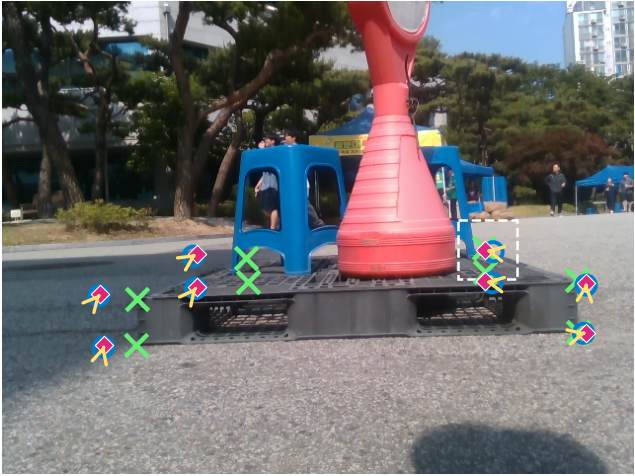
\includegraphics[width=\linewidth]{figures/example_1_frame.png} &
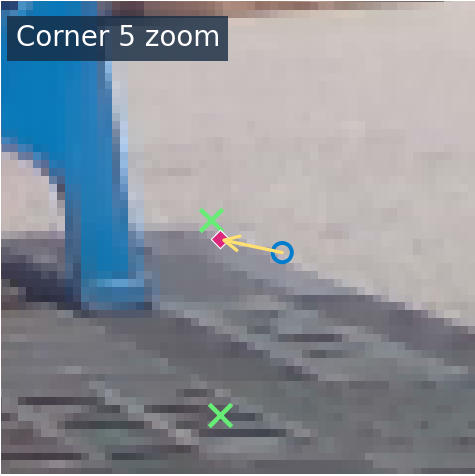
\includegraphics[width=\linewidth]{figures/example_1_zoom.png} &
\begin{minipage}[b]{\linewidth}\footnotesize
\textbf{(a) 큰 오류의 부분 감소}\\
직사각형 플라스틱, $(1.10,1.30,0.11)$m\\
Base 27.21px $\rightarrow$ N3 25.42px\\
코너 5 확대; 최대 코너 이동 8.00px\\
\texttt{eval\_pallet07}\\
프레임 \texttt{1778652125245035520}
\end{minipage}\\[4pt]
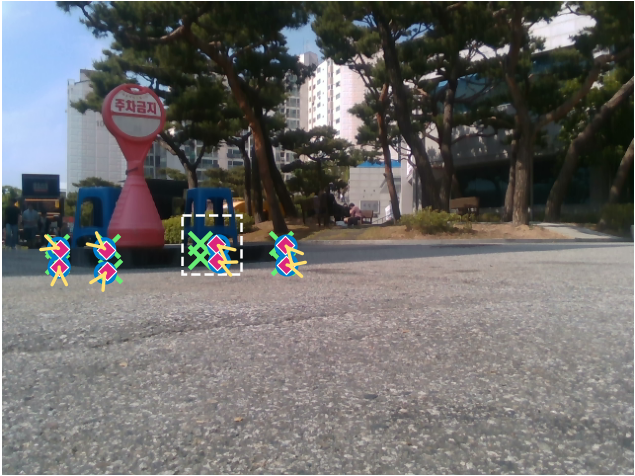
\includegraphics[width=\linewidth]{figures/example_2_frame.png} &
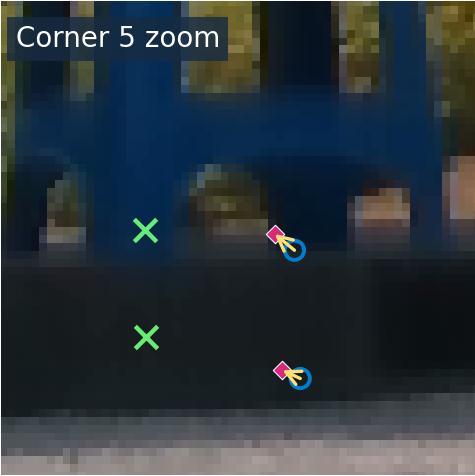
\includegraphics[width=\linewidth]{figures/example_2_zoom.png} &
\begin{minipage}[b]{\linewidth}\footnotesize
\textbf{(b) 코너 오차 감소}\\
직사각형 플라스틱, $(1.10,1.30,0.11)$m\\
Base 8.48px $\rightarrow$ N3 7.45px\\
코너 5 확대; 최대 코너 이동 3.26px\\
\texttt{eval\_pallet09}\\
프레임 \texttt{1778653706706429696}
\end{minipage}\\[4pt]
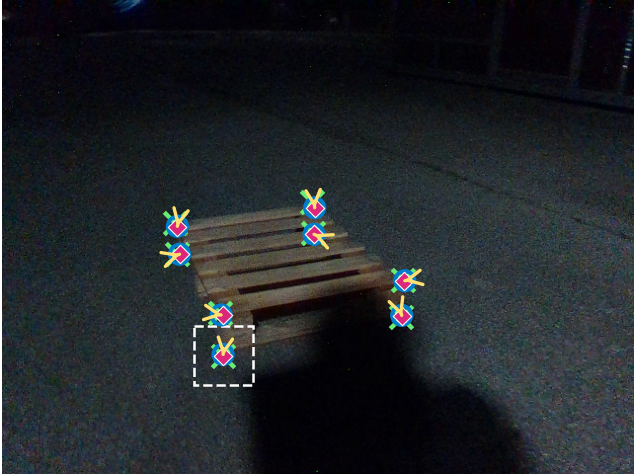
\includegraphics[width=\linewidth]{figures/example_3_frame.png} &
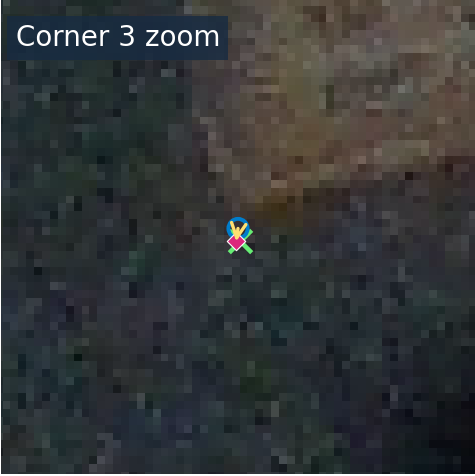
\includegraphics[width=\linewidth]{figures/example_3_zoom.png} &
\begin{minipage}[b]{\linewidth}\footnotesize
\textbf{(c) 원래 양호한 예측의 소폭 악화}\\
직사각형 목재, $(0.80,0.59,0.14)$m\\
Base 2.90px $\rightarrow$ N3 2.99px\\
코너 3 확대; 최대 코너 이동 1.66px\\
\texttt{wood\_night\_01}, 프레임 \texttt{029919}
\end{minipage}
\end{tabular}
\caption{동일한 기존 영상·좌표의 보정 예시. 그림은 고정 seed 1을 표시하고, 사례 선정에는 세 seed의 영상별 평균 코너 오차 변화가 사용되었다. 수치는 알려진 코너 0--7의 대칭 고려 영상별 평균으로 주표의 풀링 중앙값과 다르다. 원래 예시의 영상과 확대 영역을 자르고 설명 레이블만 재배치했으며 코너 위치를 변경하지 않았다. 큰 오류의 부분 감소와 소폭 악화를 함께 보존한다.}\label{fig:examples}
\end{figure*}


\subsection{추가 비용과 추정기 업데이트 대안}
주 비용 비교는 아래 표~\ref{tab:matched_runtime}의 같은 환경·동기화 벽시계 경계이다. 이전 세 기반의 CUDA event 계측은 보충자료에 별도 보존하며 YOLO 환경과 DOPE/ResNet 환경을 합쳐 비용 순위를 만들지 않는다. GPU event의 N3 head-only 중앙값과 전체 벽시계 중앙값 차이는 다른 계측량이다. 비용 수치를 Jetson 시간이나 모든 대안의 효율 우월성으로 확대하지 않는다.

표~\ref{tab:update_alternative}는 공통 플라스틱 128장으로 제한한 추정기 업데이트 대안이다. N3의 \pckten 은 56.244\%로 보정 의사 레이블 학생의 51.472\%보다 높았으며 위치·회전 중앙값도 낮았다. 합성 추가 학습과 원래 의사 레이블 학생을 포함한 대안 간 차이는 이 집합과 각 감독 예산에 한정된다. 별도 교사를 사용한 학생을 N3를 학습에 적용한 방법으로 명명하지 않으며, 자기학습 전체가 열등하거나 과적합이 실패 원인으로 확정됐다고 해석하지 않는다.
\begin{table*}[t]
\centering\footnotesize
\setlength{\tabcolsep}{4pt}
\caption{플라스틱 공통 128장에서 추정기 업데이트와 출력 보정의 비교.}\label{tab:update_alternative}
\begin{tabularx}{\textwidth}{Yrrrrr}
\toprule
경로 & \shortstack{코너 중앙값\\(px)} & \shortstack{코너 P90\\(px)} & \shortstack{\pckten\\(\%)} & \shortstack{위치 중앙값\\(cm)} & \shortstack{회전 중앙값\\(도)} \\
\midrule
Base & 9.565 & 40.902 & 49.137 & 9.353 & 3.530 \\
합성 추가 학습 & 9.741 & 41.776 & 48.629 & 9.203 & 3.507 \\
원래 의사 레이블 학생 & 9.961 & 41.958 & 47.513 & 9.226 & 3.942 \\
보정 의사 레이블 학생 & 8.954 & 42.085 & 51.472 & 9.186 & 3.766 \\
Base+N3 & 8.290 & 40.089 & 56.244 & 8.117 & 2.900 \\
\bottomrule
\end{tabularx}
\tabnote{모든 행의 집합은 128장·전체 참조 985코너·유효 예측 931코너이다. 반복 개발 부분집합이며 독립 시험이 아니다. 별도 교사와 감독을 사용한 학생을 N3 학생으로 부르지 않는다. 학습·감독 예산이 같은 단일 요인 비교는 아니다.}
\end{table*}


\subsection{같은 실행 경계의 Base/N3/PoseFix 비용}
표~\ref{tab:matched_runtime}의 주 시간은 native BGR 영상이 메모리에 있는 상태에서 전처리, 동결 검출기·공유 특징 포착, 보정기의 crop/표본화·디코더와 최종 prediction-only W/D+PnP를 모두 포함한 동기화 벽시계 시간이다. 영상 파일 decoding과 모델 loading은 제외한다. 원래 모델별 수치 계약을 유지했으며 원결과와의 점 좌표 차이는 Base/N3 0px, PoseFix 최대 0.000122px로 0.001px 검산 허용 오차 이내였다. 첫 450호출은 YOLO의 cuDNN TF32 계약 차이로 폐기했고, 정정된 450호출 중 준비 60회와 측정 390회를 구분했다. 새 학습은 0회다.
\begin{table}[t]\centering\footnotesize
\caption{같은 RTX 3080/pallet-yolo26 환경의 전체 벽시계 비용. 모델별 원래 수치 계약을 보존한 Base/N3/PoseFix 방법 전체 비교.}\label{tab:matched_runtime}
\begin{tabularx}{\columnwidth}{Yrrr}\toprule
방법 & 중앙(ms) & P90(ms) & 자세 산출 \\\midrule
Base & 11.056 & 13.081 & 130/130 \\
N3 seed 1 & 14.470 & 17.170 & 130/130 \\
PoseFix 방식 seed 1 & 25.239 & 27.311 & 130/130 \\
\bottomrule\end{tabularx}
\tabnote{13세션의 고정 26프레임, batch 1, arm별 준비 20회와 프레임당 5반복. 같은 최종 PnP까지 포함한다. 파일 decoding·모델 loading 제외. CUDA/head-only 수치와 구분한다. 모든 모델이 동시에 resident한 process memory peak는 독립 방법별 메모리 비교에 쓰지 않는다. 출처: 새 RUNTIME\_MATCHED/RUNTIME\_VERIFICATION.json.}
\end{table}


